
\section{Related Work}	

 For computing the midsurface, this work uses feature-based techniques in the domains of simplification/defeaturing, generalization/abstraction, cellular decomposition and topological validation. Following sub-sections evaluate some of the relevant past works in these domains and try to extract specific issues for addressal in this research.
 
 \subsection{Midsurface}
 
Midsurface is a special case of a more generic structure called ``Medial Object''. Medial Object is the geometry that is mid-way inside an input shape. The input shape can be an image, a 2D profile or a 3D solid. One of the early works in the field of Medial object was by a theoretical biologist, Harry Blum in 1967 \cite{Harry1967}. Some of the most researched techniques are  Medial Axis Transform (MAT), Chordal Axis Transform (CAT), Thinning, Pairing (Medial Abstraction, MA), etc. (Figure \ref{fig:medials}). Two of the most popular techniques amongst them  are MAT and MA. 

	\begin{figure} [!h]
		\centering
		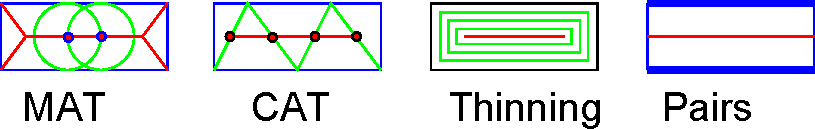
\includegraphics[width=0.8\linewidth]{..//Common/images/MedialMethodsOnlyShort.pdf}
		\caption{Medial Computation Techniques}
		\label{fig:medials}
	\end{figure}



MAT is a locus of the center of an inscribed maximal disc as it rolls around the object's interior. As a formal definition is available, it can be generated for any shape, but the major drawback of this technique is that it creates unnecessary branches and gives unpredictable output due to perturbations on the input shape.

MA\added[remark={Reviewer 1 (4): The authors are requested to consider the following papers to add to their survey, Mohesen Rezayat \ldots}]{, initiated by Rezayat \cite{Rezayat1996},}  involves identifying ``face pairs'', constructing midsurface patches for each and then building a connected midsurface by \replaced[remark={Reviewer 1(5): Please reconsider the sentence structure. (e.g. extend-trim-sweING may be changed?}]{extending or trimming and then joining}{extend-trim-sewing} the patches. This surface-pairing approach has benefits over MAT techniques because the resultant geometry is cleaner and requires lesser post-processing \cite{Lockett2008}. It has difficulty in identification of the surface pairs as well as in joining the midsurface patches. Many of the commercial CAD-CAE packages use this approach and thus, have to provide manual/semi-automatic methods to correct the failures.

\deleted[remark={Author: Reduced for brevity}]{Feature-based approaches leverage the use of feature information in the computation of the midsurface.  Information readily available in the feature has been used by few to compute midsurface patches \cite{Robinson2006} \cite{DengBrittonLamTorMa2002}, whereas few others work on the final solid shape, recognize features  after decomposition and then create the midsurface \cite{Chong2004} \cite{Boussuge2013} \cite{Boussuge2013a} \cite{Woo2013}. The work done so far seems limited to very basic shapes and interactions.}
 
 \subsection{Defeaturing/Simplification}
 
Defeaturing indicates removal of unwanted features.  Thakur et al. \cite{Thakur2009} surveyed and classified various techniques used till then, into categories such as surface-based, volume-based and feature-based.  The research presented  here proposes a feature-based defeaturing technique which computes the ``gross shape'' (similar to the original shape but with far lesser details) \cite{YogeshIITM2013}. It does not take into account the usual CAE inputs such as load paths, boundary conditions, symmetry, etc., thus making it suitable even for other operations like shape matching, retrieval, etc. CAE inputs can also be integrated on top as per the requirements. \deleted[remark={Author: Reduced for brevity}]{After defeaturing, the model gets simplified and results in the gross shape for which the computation of midsurface is far more effective \cite{YogeshCADConf2015}}.
 
Dabke \cite{Dabke1994} through the concept of ``global idealization'', was one of the first researchers to leverage the feature information for defeaturing. \deleted[remark={Author: Reduced for brevity}]{His technique was based on heuristic rules derived from the analyst's experience but was rudimentary in the range of usages.} Lee \cite{SangHunLee2005} elaborated a technique to reorder features in the history tree and then build partly up to a given level of simplification. \deleted[remark={Author: Reduced for brevity}]{One of the major limitation was that the use of cellular model removed the feature update capability.} Russ \cite{Russ2012} decided suppressibility on the feature type, feature dimensions, proximity of features to the boundary conditions, analysis type and part dimensions. Commercial packages like ACIS\textsuperscript{\textregistered}, Autodesk Fusion\textsuperscript{\textregistered}, Altair's Hypermesh\textsuperscript{\textregistered},  etc. also provide similar defeaturing capabilities mainly for CAE analysis, but have to do heuristic feature recognition first, which is prone to failures.
	
\subsection{Feature Abstraction}
Features, not only carry shape information (geometry and topology) but also embed meta-information based on the application context. With a variety of applications, each having their own needs,  has resulted into various {\em feature-schemes}.  This makes writing a  generic/portable feature-based algorithm, a humongous task. Abstraction alleviates this problem by the extraction of a generic feature-form from various specific features. 
 
  Middleditch  provided feature abstraction by proposing structure, construction sequence and point-set, so as to separate issues of  solid modeling, feature modeling and constraints \cite{Middleditch1997}.  Tessier tried to formulate features in terms of generic attributes such reference attributes for reference planes, parameter attributes for model type, depth, etc.\cite{Tessier2013}. 
  
From the research reviewed so far, it appears that there is no feature abstraction schema, generic enough to represent the CAD form features. This research attempts to propose one, by  abstracting form features as generic as a Loft feature, with profiles and a guide curve.
  
 \subsection{Cellular Decomposition}
 
Cellular decomposition, in the context of the current research, is the division of a feature-based CAD model into non-volumetrically overlapping, but surface-overlapping sub-solids (called ``cells'').  Research in  cellular decomposition, especially for Computer-aided Manufacturing (CAM) and CAE has been going on for decades. Feature-based cellular decomposition, which deals with either decomposition of features, or feature-recognition after decomposition,  has also been  researched extensively \cite{Bidarra1993,Woo2003, Boussuge2013}. There have been a few attempts to compute a midsurface using cellular-decomposition as well \cite{Chong2004, Woo2013, Boussuge2013, Zhu2015}, but the methodologies presented therein appear to be limited due to extensive use of heuristic rules such as hard-coded values for detecting edge/face pairs, support for limited types of geometries, only limited scope in terms of the range of connections  handled, etc.

\added[remark={Reviewer 1:  In comparison to the models shown in recent work \cite{Woo2013} }]{For example, Woo's \cite{Woo2013} approach, uses face-pairing using distance criteria, which may generate incorrect pairs. It is restricted to only analytical surfaces and only parallel face-pairs.}

%Chong et al. \cite{Chong2004} split the solid model into sub-volumes which, in turn, extracted their own midsurface patches. Kageura's \cite{Kageura2009} US Patent 2009/0271156 A1 proposed to partition the input model first, generate the adjacency information and then extract the midsurface patches.  Cao \cite{Cao2009} \cite{Cao2011} decomposed the final solid and recognized additive remnant swept primitives, got their sketches, computed midcurves for edge-pairs and created midsurface patches but the joining logic was not much elaborated. Boussuge et al.  \cite{Boussuge2013,Boussuge2013a}  split the solid body at concave edges, recognized (only) positive  protrusion features in the sub-volumes and then idealized each to a midsurface with a joining logic restricted to only a couple of hard-coded interaction types. Woo \cite{Woo2013} used his maximal volume technique \cite{Woo2006, Woo2009} and computed midsurface for each sub-volume using face-pair technique. It worked only for analytical surfaces and parallel face pairs.

\subsection{Analysis of the Survey Findings} \label{sec:litsurvey:analysis}
 
 After analyzing various past approaches, both in the academic and commercial domains, it was concluded that there has been limited success in the computation of a well-connected midsurface. \deleted[remark={Author: Reduced for brevity}]{Many approaches are heavily heuristic, non-generic and need post-processing like pruning erroneous branches, extending-trimming to join gaps, removing overlapping surfaces, etc.}
  \added[remark={Reviewer 2: Several commercial software such as MSC Apex already implemented tools for modeling midsuface. For example, Smart MidSurface is developed by MSC Software. Smart MidSurface can accelerate mid-surface modeling to validation.}]{Commerical packages like Autodesk Inventor\textsuperscript{\textregistered}, MSC's Smart Midsurface\textsuperscript{\textregistered}, Altair's Hypermesh\textsuperscript{\textregistered}, etc. provide automatic midsuface functionality, but they appear to result in disconnected midsuface, especially for the non-trivial parts, and require manual patching to get them connected}. By far, the most widely-used \added[remark={Associate Editor: Please clarify how the proposed approach is different from the implementations in commercial CAD systems}]{commercial} approach appears to be the Midsurface Abstraction (Face Pairing), but even that also is not devoid of issues.  Two of the most critical problems are elaborated below:
	

\begin{itemize}[noitemsep,topsep=2pt,parsep=2pt,partopsep=2pt]%leftmargin=*
	\item  \textbf{Face Pairs Detection Problem}:  \label{sec:facepairdetection}
In MA, each face-pair computes its own midsurface patch. Finding the face-pairs in a complex part is very challenging \cite{Boussuge2013}. This research addresses this problem by using the feature-information for computation of patches and avoids detection of face-pairs. \deleted[remark={Author: Reduced for brevity}]{Here, due to a large number of feature types, writing midsurface-computation for all the feature types separately becomes a tedious task. The solution proposed for this issue is to abstract/generalize these individual feature types into some generic form and then compute midsurface patches for just the generic type.} Feature abstraction, called $\mathcal{ABLE}$, has been proposed to generalize various form-features into a generic ``Sweep/Loft'' feature having a profile and a guide curve. Midsurface patch can then be computed by sweeping midcurve of the profile along the guide curve (more details in section \ref{sec:scell}) \cite{YogeshIITG2014}.

	\item  \textbf{Face-Pair Interaction Problem}: \label{sec:facepairinteraction}
Midsurface patches need to be connected \replaced[remark={Reviewer 1(5):  ``In a similar manner similar to'' should be ``in a manner similar to''}]{in a manner similar to}{in a similar manner similar to} how the face-pairs in the input model are connected. As there is no theoretical framework encompassing all the possible interaction types, providing a unified logic has not been possible \cite{Stolt2006}.   \deleted[remark={Author: Reduced for brevity}]{Developing a connection logic for each of these types separately can be a tedious task.} This research proposes  leveraging of feature-based cellular decomposition to decompose the given solid into sub-volumes and then devise a generic logic for joining the midsurface patches (more details in section \ref{sec:icell}).
\end{itemize}
 
